\section{Постановка задачи машинного обучения}

Одним из первых, кто дал определение предмету машинного обучения стал американский ученый Артур Самуэль. В 1959 году в своей работе \cite{Samuel:ML}, посвященной созданию искусственного интеллекта по игре в шашки с помощью алгоритма minimax, Артур Самуэль дал определение тому, что есть машинное обучение -- процесс обучения, в результате которого компьютеры способны показывать поведение, которое в них явно не было заложено.

Более современное и точное определение дал Том Митчелл в 1998 году. Корректно поставленная задача обучения определяется следующим образом: говорят, что компьютерная программа обучается на основе опыта E (experience) по отношению к некоторому классу задач T (task) и меры качества P (performance), если качество задач из T измеренное на основе P, улучшается с приобретением опыта E.

Большинство алгоритмов машинного обучения условно можно разбить на 2 класса: обучение с учителем (supervised learning) и обучение без учителя (unsupervised learning).

В алгоритмах обучения с учителем подразумевается обучение на размеченных данных, то есть когда дана матрица, описывающая объекты с помощью признаков (матрица ''объекты-признаки'') и вектор ответов для каждого объекта. Таким образом методы обучения с учителем можно представлять как функциональную зависимость: на каждый набор признаков $x \in X$ есть ответы $Y$ такой, что $y:~X \rightarrow Y$, где $y$ -- искомая зависимость.

Рассмотрим такой подход более подробно \cite{coursera:voroncov}. Пусть $X$ -- множество объектов, $Y$ -- множество ответов, $y:~X \rightarrow Y$ -- неизвестная зависимость (target function).

Пусть также нам известны:\\
\begin{description}[font=$\bullet$]
    \item $\{ x_1, \dots, x_l \} \subset X $ -- известное подмножество объектов;\\
    \item $y_i = y(x_i),~~\forall~i=\overline{1,n}$ -- известное множество результатов.\\
\end{description}
Ставится задача найти $a:~X \rightarrow Y$ -- искомый алгоритм (decision function).

Замечание: как правило множество объектов описывается с помощью признаков. Пусть есть $n$ объектов, тогда под признаками объекта будем иметь в виду следующее отображения: $f_j:~X \rightarrow D_j,~~\forall~j=\overline{1,n}$.\\
Признаки могут быть: количественными $D_j=\mathbb{R}$, бинарными $D_j=\{A, B\}$, номинальными $|D_j|=k<\infty$, упорядочено номинальными. Один объект может задаваться набором признаков разных типов.

Тогда объект $x \in X$ может быть описан вектором признаков $f_1(x), \dots, f_n(x)$.
Следовательно, все объекты можно описать с помощью матрицы ''объекты-признаки'' (feature data):
$$ F = 
\begin{pmatrix}
f_1(x_1) & f_2(x_1) & \dots & f_n(x_1) \\
f_1(x_2) & f_2(x_2) & \dots & f_n(x_2) \\
\dots    & \dots    & \dots & \dots    \\
f_1(x_l) & f_2(x_l) & \dots & f_n(x_l) \\
\end{pmatrix}
$$
Каждой строчке соответствуют правильные (ожидаемые) ответы, полученные в результате эксперимента, наблюдения, опроса и т.д. По типу представления множества ответов можно разбить на 3 класса:
\begin{description}[font=$\bullet$]
    \item классификация: $Y=\{A,B\},~Y=\{A_1,\dots,A_k\},~Y\{A,B\}^k$;
    \item регрессия: $Y=\mathbb{R},~Y=\mathbb{R}^k$;
    \item ранжирование: $Y$ -- конечное упорядоченное множество.
\end{description}

Предсказательная модель $a(x)$ строится как параметрическое семейство функций над некоторой фиксированной функцией $g(x)$. Более формально модель $A = \{ a(x) = g(x,\theta) | \theta \in \Theta \}$, где $g:~X \times \Theta \rightarrow Y$ -- фиксированная функция, $\Theta$ -- множество допустимых параметров $\theta$.


В обучении без учителя данные об ответах неизвестны, поэтому можно говорить лишь о том как данные расположены друг относительно друга, данный метод машинного обучения происходит без участия экспериментатора и применяется для обнаружения внутренних взаимосвязей. Обычно так решаются задачи кластеризации, понижения размерности, визуализации данных.

Также используются методы обучения с подкреплением (reinforcement learning), когда набор данных дается из некоторого потока, а также рекомендательные системы (recommender systems).

Существуют задачи частичного обучения, которые занимают промежуточное положение между задачами регрессии и задачами кластеризации. Задача возникает когда только на части обучающей выборки даны ответы, а другая часть неразмечена, обычно такие задачи возникают при больших объемах данных, когда разметить всю выборку либо невозможно, либо очень дорого. При этом задачи частичного обучения не сводятся ни к классификации, ни к кластеризации.


\section{Методология решения задач машинного обучения}

Вне зависимости от метода машинного обучения задача состоит из 2-х этапов: обучение и применение.
На первой стадии происходит построение оптимального алгоритма $a$ -- функция, дерево, набор инструкций и др. На второй стадии алгоритм выдает ответы для новых объектов.

Оптимальным алгоритмом будем называть такой алгоритм, который на большинстве объектов обучающей выборки дает правильные ответы или достаточно близкие ответы к ожидаемым. Для того чтобы это сделать нужно определять точность или расстояние между объектами, другими словами нужно задать метрику в пространстве объектов. Для этого вводится понятие функции потерь $\mathfrak{L}$ -- величина ошибки алгоритма $a \in A$ на объекте $x \in X$:
\begin{description}[font=$\bullet$]
    \item $\mathfrak{L} (a,x)=[a(x) \neq y(x)]$ -- индикатор ошибки для случая классификации;
    \item $\mathfrak{L} (a,x)= (a(x) - y(x))^p$ -- для случая регрессии.
\end{description}
Замечание: при $p=1$ для регрессии функция ошибки берется как модуль разности алгоритма и ответа.

На практике для случая регрессии обычно берут $p=2$ т.к. при $p=1$ возникает проблема с дифференцированием функции потерь. 

Чтобы оценить алгоритм в целом берут деленную на размер сумму функций потерь, получившуюся величину называют эмпирическим риском (функционал качества алгоритма $a$ на объектах $X^l$): $Q(a, X^l) = \dfrac{1}{l}\sum\limits_{i=1}^{l}\mathfrak{L}(a,x_i)$.

Таким образом задача обучения сводится к задаче оптимизации (минимизация эмпирического риска на обучающей выборке): $\mu(X^l) = \arg\min\limits_{a \in A} Q(a,X^l)$.\\
Замечание: иногда сумму делят не на $l$, а на $2 \cdot l$, с той целью, чтобы при дифференцировании функции эмпирического риска сократились некоторые коэффициенты (для $p=2$).

Для решения задачи минимизации применяют различные численные методы. Например, метод наименьших квадратов (МНК).


\subsection{CRISP-DM}

\begin{wrapfigure}{r}{0.45\linewidth} 
    \vspace{-2ex}
    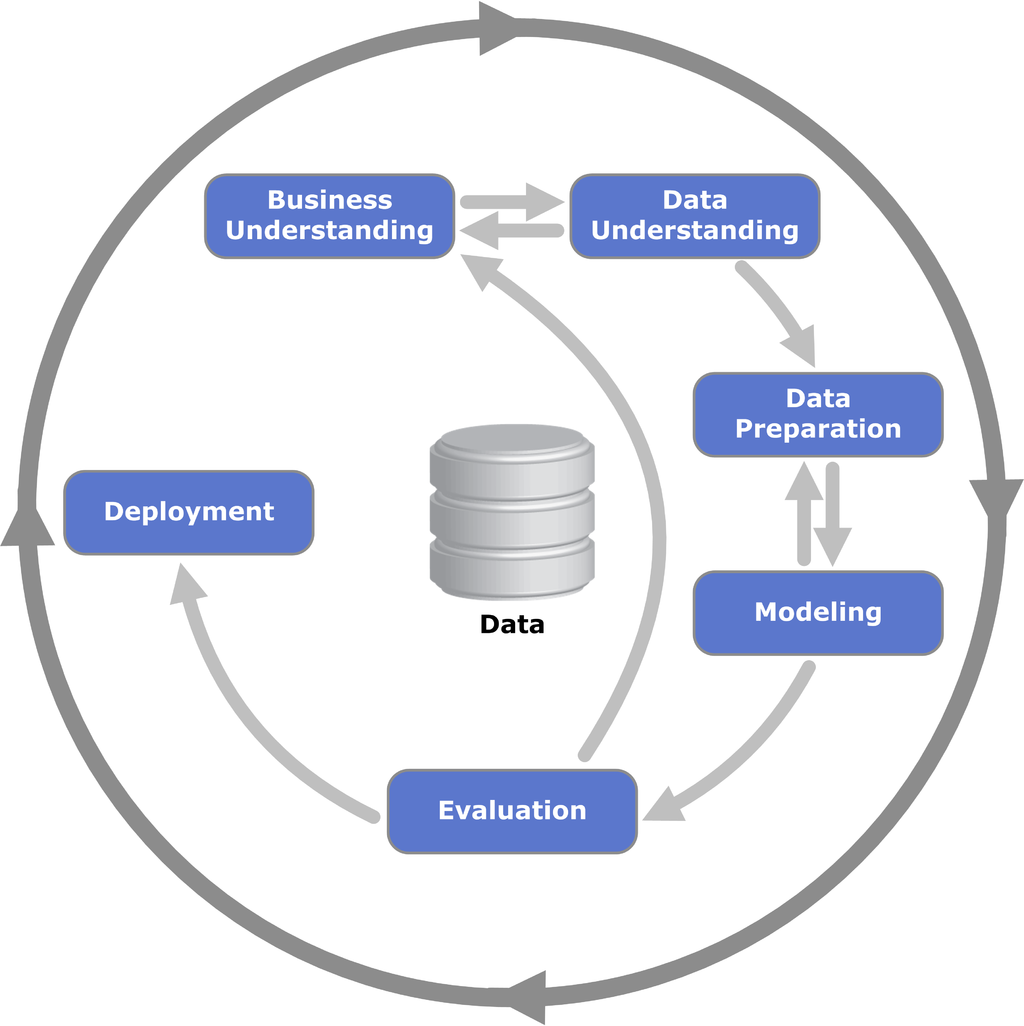
\includegraphics[width=\linewidth]{src/img/CRISP-DM_process_diagram.png}
    \caption{Жизненный цикл исследования данных \cite{wiki:crisp_dm}}
    \label{fig:crisp_dm}
\end{wrapfigure}

Таким образом, любая задача машинного обучения: классификация, регрессия, кластеризация сводится к оптимизационной задаче, возможно с ограничениями. Что приводит к большому множеству методов машинного обучения, чтобы облегчить процесс решения задач, был разработан и предложен CRISP-DM (CRoss Industry Standard Process for Data Mining) -- межотраслевой стандарт решения задач интеллектуального анализа данных. CRISP-DM -- модель жизненного цикла исследования данных.
Первая версия данного стандарта была принята в 1999 году. Стандарт призван формализовать схему решения задач анализа данных. Предполагается алгоритм решения произвольной задачи анализа данных в 5 шагов, причем они могут замыкаться в цикле.

\begin{enumerate}[label=\arabic*.]
    \item В начале исследователь должен понять предметную область или сферу бизнеса;
    \item Далее необходимо понять как собирались данные;
    \item На следующем шаге нужно определить есть ли в данных шумы, пропуски, выбросы, все ли признаки несут полезную информацию, можно ли вычислить полезные признаки по уже имеющимся, данный этап можно назвать подготовкой данных;
    \item После происходит моделирование или построение предсказательной модели;
    \item Полученная модель оценивается с помощью выбранных метрик;
    \item Если качество полученной модели удовлетворяют исследователя, модель внедряется в производственные процессы и эксплуатируется.
\end{enumerate}
Помимо CRISP-DM существуют менее известные стандарты: My own, SEMMA и другие. На сайте \cite{poll:crisp_dm} публикуются результаты опросов по популярности методологий анализа данных.



\section{Теория оптимизации}

Во многих задачах науки, экономики и бизнеса возникают проблемы нахождения экстремальных значений целевой функции. При этом на множество допустимых решений могут быть наложены ограничения. Такие задачи называются задачами оптимизации, если есть ограничения, то говорится о задаче условной оптимизации, безусловной оптимизации. Рассмотрим некоторые методы решения задач оптимизации.

\subsection{Градиентный спуск}

Метод градиентного спуска является наиболее часто используемым методом ввиду быстроты работы для большинства задач и многообразия модификаций метода (метод наискорейшего спуска, метод сопряженных градиентов, метод Нестерова, метод стохастического спуска и многие другие)
Для отыскания экстремальной точки в градиентном спуске используют итеративную формулу:
$$ x := x - \alpha \nabla f(x) $$
Где $\nabla f(x)$ -- градиент функции $f(x)$, в векторной форме градиент можно записать как $\nabla f(x) = \frac{\partial f(x)}{\partial x_1} \vec{i_1} + \frac{\partial f(x)}{\partial x_2} \vec{i_2} + \dots + \frac{\partial f(x)}{\partial x_n} \vec{i_n}$. Направление градиента указывает на то направление из точки $x$, которое имеет наибольшую скорость роста функции из данной точки. Соответственно, $-\nabla f(x)$ показывает направление наискорейшего убывания;

$\alpha$ -- шаг градиента (в машинном обучении называют скоростью обучения). Данный параметр выбирается вручную, при этом, если $\alpha$ мал, то методу потребуется много итераций для сходимости, если же $\alpha$ большое, то метод градиентного спуска может начать расходится, то есть значение $x$ будет отдалятся от точки экстремума. Существует условие Липшица, которое дает достаточное условие сходимости градиентного спуска: если $\exists L:~\forall x, y \hookrightarrow || \nabla f(x) - \nabla f(y) || \leq L || x - y ||$, то $\forall \alpha < \frac{2}{L}$ гарантируется убывание функции $f(x)$. На практике обычно выбирают $\alpha=10^{-2}$, либо еще меньше в зависимости от того, какая точность необходима.

\begin{wrapfigure}{r}{0.45\linewidth} 
    \vspace{-3ex}
    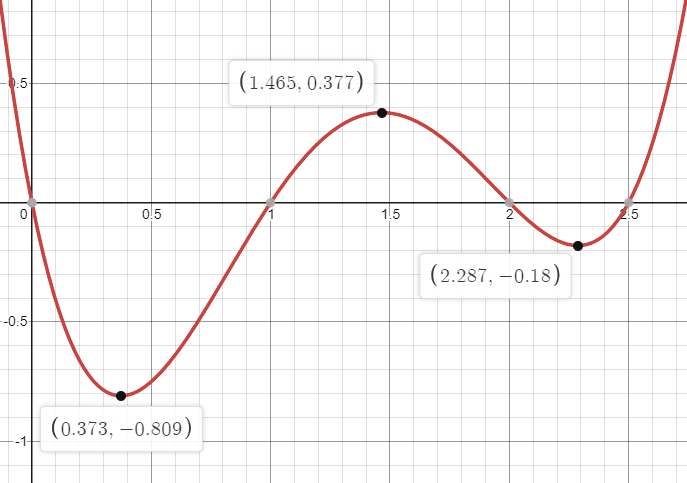
\includegraphics[width=\linewidth]{src/img/multi_extreme.png}
    \caption{Проблема много экстремальности функции}
    \label{fig:multi_extreme}
\end{wrapfigure}

Важной особенностью градиентных методов является выбор начального приближения $x_0$, так, если производится поиск минимума и функция имеет несколько минимумов, как на рисунке \ref{fig:multi_extreme}, то выбор $x_0$ будет определять найденный минимум. Например, если $x_0 = 2$, метод найдет минимум $f(x^*) = -0.18$, если $x_0 = 1$, то $f(x^*) = -0.809$, если же $x_0 = 1.5$, то метод не сможет найти ни один минимум функции, поскольку в точке $x = 1.5$ производная функции $f(x)$ равна 0, поэтому $\nabla f(x) = 0$ и формула градиентного спуска вырождается в $x := x$. Для того чтобы метод искал глобальный минимум можно запустить данный метод несколько раз из разных начальных точек. Выбрать начальные приближения можно как самому, так и выбрать их случайным образом из равномерного распределения на отрезке $[ a, b ]$. Для проверки того, что был найден глобальный минимум можно запустить метод из точек $x^* - x_L,~x^* + x_L$, где $x^*$ -- найденный минимум, $x_L$ -- точка с большими по модулю координатами. Если метод не сойдется к тому же решению, то необходимо сравнить 2 минимума и выбрать наименьший.

При поиска экстремума в овражных функциях градиентный спуск сходится медленно, причем если число аргументов функции велико, то довольно часто можно встретить овражные области. Для решения данной сходимости используют модификации градиентного спуска, так называемые овражные методы.

Для ускорения сходимости градиентного спуска применяют различные техники: можно определять $\alpha$ на каждом шаге по следующей формуле: $\alpha_{k} = \arg \min\limits_{\alpha \in \left[  0, \infty \right) } f(x^k - \alpha_{k-1} f'(x_k))$ метод с таким выбором градиентного шага носит называние метод наискорейшего спуска, также можно уменьшать параметр $\alpha$ на каждом шаге, идея заключается в том, что после каждого шага расстояние до экстремума уменьшается, следовательно, нужно уменьшить градиентный шаг.


\subsection{Инерционный градиентный спуск}

Метод известен с середины 20 века и изначально носил название метод тяжелого шарика. Идея данного метода -- добавить в формулу градиентного спуска свойство инерционности, то есть чтобы на каждом следующем шаге аргумент $x_{k+1}$ зависел не только от значения антиградиента, но и также от значения предыдущего шага. Для этого предлагается добавить в формулу градиентного спуска следующее слагаемое $\beta (x_k - x_{k-1})$, где $\beta$ -- коэффициент инерции, также как и $\alpha$ является гиперпараметром, то есть задается вручную. Как правило коэффициент инерции берется немного меньше единицы.

Все семейство инерционных градиентных методов можно описать следующей формулой:
$$ x_{k+1} = x_k - \alpha_k \nabla f(x_k) + \beta_k (x_k - x_{k-1}) $$

Дополнительное слагаемое не меняет асимптотической сложности алгоритма, при этом правильном выборе параметров $\alpha_k, \beta_k$ можно добится ускорения метода на порядок.


\subsection{Стохастический градиентный спуск}

Идея метода заключается в использовании вместо градиента функции $\nabla f(x)$ другую функцию (случайный процесс) $g(x,\theta)$ такую, что математическое ожидание $E[g(x,\theta)] = \nabla f(x)$, где $\theta$ -- случайная величина.
Метод стохастического градиента можно описать следующей формулой:
$$ x_{k+1} = x_k - \alpha_k g(x_k,\theta_k) $$

Если $x$ -- вектор с большим количеством компонент, то вычисление градиента может происходить продолжительное время. Поэтому если использовать метод стохастического градиента и в качестве $\theta$ взять случайный индекс у $x$, то есть $x_i$, где $i$ -- случайная величина, то вычисление градиента сведется к вычислению частной производной по аргументу со случайным индексом. За счет этого происходит существенное ускорение сходимости, это называется процедурой Роббинса-Монро и Кифера–Вулфовица, представленные в 1951 и 1952 годах соответственно \cite{wiki:stochastic_grad}. В настоящее время данный метод активно применяется в алгоритмах машинного обучения и в нейронных сетях, где количество признаков у объектов может быть велико. Следует сказать, что данный метод реализован в крупных библиотеках машинного обучения: TensorFlow, PyTorch, метод используется для обучения моделей с большим и сверх большим объемом данных из-за того, что даже на небольшой подвыборке объектов модель может хорошо обучиться.


\subsection{Нормальное уравнение (Normal Equation)}

Нормальное уравнение позволяет найти экстремум функционала аналитически, без необходимости применять итеративный подход. Пусть функционал задан следующим образом: $\mathcal{L}(\theta_1,\theta_2,\dots,\theta_m) = \frac{1}{2m} \sum\limits_{i=1}^{m}(h_{\theta}(x^{(i)}) - y^{(i)})^2$ поставим задачу минимизации этого функционала по всем параметрам $\theta$, при условии, что известны $m$ пар $(x^{(i)}, y^{(i)})$. Составим из $x^{(i)}$ матрицу: $X = (x^{(1)}), x^{(2)}, \cdots, x^{(m)}$, тогда $\theta = (X^{T} X)^{-1} X^{T} y$.

В отличии от градиентных методов в данном методе не нужно проводить итерационную процедуру, а также в методе отсутствуют гиперпараметры. Однако для вычисления ответа нужно вычислить обратную матрицу порядка $n \times n$, алгоритм вычисления обратной матрицы работает за $O(n^3)$ по времени, поэтому для объектов с большим числом признаков, например $n=10^6$ потребуется $C \cdot 10^{18}$ операций, где $C$ -- некоторая константа из алгоритма обратной матрицы. Современные компьютеры могут обрабатывать порядка $10^9$ операций в секунду, учитывая нужное количество операций алгоритм не успеет за разумное время вычислить минимум функции. Поэтому область применимости метода -- объекты с небольшим числом параметров $(< 10^4)$. На объектах с большим числом признаков хорошо работает стохастический градиентный спуск.


\section{Регрессионный анализ}


\subsection{Линейные модели}

\subsubsection{Линейная регрессия}

\subsubsection{Полиномиальная регрессия}

\subsubsection{Пуассоновская регрессия}

\subsubsection{Геометрическая регрессия}

\subsubsection{Проблема переобучения}

Пример линейной модели\\

Эмпирические оценки обобщающей способности\\
* Эмпирический риск на тестовых данных (Hold-out)\\
* Скользящий контроль (leave-one-out)\\
* Кросс-проверка (cross-validation) по N разбиениям\\

\subsection{Нелинейные модели}

\subsubsection{Градиентный бустинг}

\subsubsection{Решающие деревья}

\subsubsection{Случайный лес}
